\subsection{The Scale Cube in Ethereum}

The Scale Cube, as in \autoref{fig:scale-cube}, uses the representation of a
cube drawn on a 3-dimensional Cartesian space to define three different scaling
directions an architecture can develop in order to growth and shrink along with
the demand. Although in a Cartesian space we could measure the cube size, the
Scale Cube does not provide actual metrics to quantify the scalability, but
rather a way of think about scale; that is what we mean with \emph{scaling
directions}.

\begin{figure}
	\begin{center}
		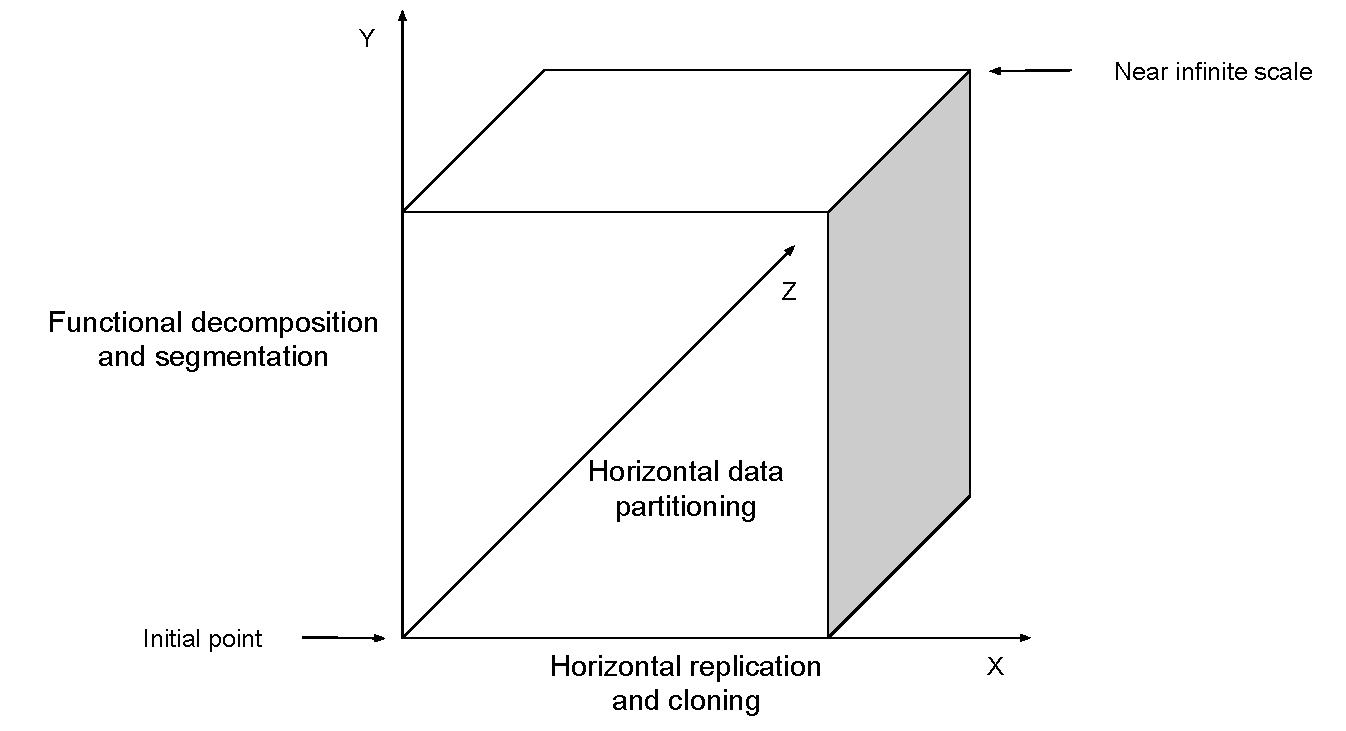
\includegraphics[width=0.8\textwidth]{./res/img/scale-cube.pdf}
	\end{center}
	\caption{The Scale Cube.}
	\label{fig:scale-cube}
\end{figure}

The use of one or two axes does not preclude the possibility to scale on the
third axis. The initial point with coordinates $(0,0,0)$ means least
scalability. The prototypical system at the initial point consists of a single
monolithic application and storage retrieval system likely running on a single
physical machine~\cite{bib:art-of-scalability}. Of course, it might scale up,
that is it could run on a more powerful machine, but it won't scale out, then it
will not take advantage of a distributed architecture. All of the three axes
scales well from a transaction perspective, that is, in our case, the
transaction throughput. % TODO check this last sentence